% English version of paper/ja_v3/01_序論.md (ver3 draft 2, 2026-11-17). Structure of Ishii et al. 2022: field -> prior work -> However -> this study -> research questions and Fig. 1 -> "First, we analyze ... Second, we propose ... This method is motivated by ..." -> section guide. No contribution list (the research questions play that role; Ishii 2022). The scoped novelty statement is in Sect. 2.5 and the conclusion.
\section{Introduction}\label{sec:intro}

Multimodal emotion recognition (MER) estimates a speaker's emotion from the voice, face and words of the same utterance. Emotion corpora differ in environmental noise, recording devices, acted versus natural elicitation and speaker demographics \cite{gideon2021addog}, and also in how they were annotated. Emotion classifiers trained on one corpus have been reported to perform worse on other corpora \cite{ryumina2025,gideon2021addog}. Many methods for fusing modalities have been proposed, including for sentiment polarity \cite{zadeh2017tfn,mittal2020m3er,yu2021selfmm,yun2024telme}, and they have been evaluated by training and testing within one corpus; Ryumina et al.\ \cite{ryumina2025} noted that 12 recent methods evaluated on IEMOCAP, MOSEI, MELD or AFEW had not been evaluated across corpora. Using MER on utterances of a corpus not used for training requires adapting the classifiers to that corpus (the target).

Labels of naturally expressed emotions are collected from several raters who watch or listen to each utterance, which is costly to repeat for every new corpus \cite{parthasarathy2020ladder,abdelwahab2018dann}, whereas unlabelled utterances are easy to collect \cite{abdelwahab2018dann}. Adapting classifiers with labelled utterances of other corpora (sources) and unlabelled target utterances or a few target labels has mainly been studied for speech emotion recognition \cite{abdelwahab2018dann,gideon2021addog,feng2023}. The multimodal cross-corpus evaluations of Ryumina et al.\ \cite{ryumina2025} and Lian et al.\ \cite{lian2026merbench} did not use target labels, and He et al.\ \cite{he2025m4ser}, who addressed a setting with a few target labels, used audio and transcribed words. In MER, the other modalities of the same utterance can also be used as information attached to unlabelled utterances. Albanie et al.\ \cite{albanie2018} attached the predictions of a facial classifier to unlabelled videos and trained an audio emotion classifier towards them, and Zhang et al.\ \cite{zhang2021combining} combined training towards targets that include predictions of other modalities with semi-supervised learning. We call the four-emotion probabilities that classifiers including other modalities assign to unlabelled utterances \emph{pseudo-labels}, and retraining a classifier towards them without temperature \emph{distillation} \cite{hinton2015distilling,albanie2018}.

However, whether these findings hold in cross-corpus MER with only a few target labels per emotion is unknown. First, studies using sources and unlabelled utterances have compared the performance of methods, but which part of the classifier error these information sources and the other modalities correct has not been measured separately in one setting. Second, Albanie et al.\ and Zhang et al.\ did not evaluate this setting, so which classifiers distillation improves, and when, is unknown. Third, audio and visual classifiers have been reported to recognise different emotions well within one corpus \cite{busso2004}, but whether this holds when classifiers trained on source corpora are applied to a target, and if so how much weight each of the audio, visual and text classifiers should receive when their predictions are combined, has not been reported.

We consider a target with only K labels per emotion. The data available in this case, which we call information sources, are labelled source utterances, the K target labels, unlabelled target utterances and the other modalities of the same utterance; the first three form the setting of semi-supervised domain adaptation \cite{saito2019mme}. We place linear emotion classifiers on features of frozen pretrained audio, visual and text encoders and split their error into the part where predictions are biased towards some emotions (\emph{answer bias}) and the part that remains after removing that bias (\emph{remaining error}). Linear classifiers on frozen features serve as a setting for measuring what each information source changes in a classifier, not as a proposed classifier architecture, and we do not claim that the results hold for fine-tuned encoders (Sect.~\ref{sec:limitations}). We answer three research questions (Fig.~\ref{fig:questions}).
\begin{itemize}
\item \textbf{RQ1(a):} Does each of the four information sources correct the answer bias or the remaining error?
\item \textbf{RQ1(b):} Does distillation raise the UAR of the audio, visual and text classifiers and of the classifier on their concatenated features (AVT)? Which classifiers gain, and when?
\item \textbf{RQ2:} How should the predictions of the audio, visual and text classifiers be combined to raise the UAR of the pseudo-labels?
\end{itemize}

\begin{figure}[t]
\centering
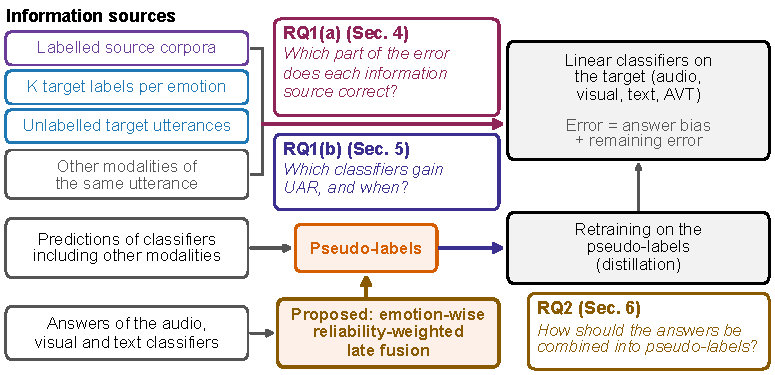
\includegraphics[width=\textwidth]{figures/fig_v2_questions_en.pdf}
\caption{The three research questions, written on the arrows of the processing flow they ask about}\label{fig:questions}
\end{figure}

First, we analyse in three settings with different numbers of source corpora which part of the error each information source reduces, to address RQ1(a) and RQ1(b) (Sect.~\ref{sec:analysis}). For audio classifiers with one source corpus (K = 5), label-free feature-mean subtraction obtained 4.69\pt\ of the 5.26-point gain of training on the source and the K labels together. With all non-target corpora as sources, the remaining error was reduced in 7 of 210 conditions by eight methods that use same-modality unlabelled utterances and in 38 of 81 conditions by distillation on pseudo-labels including other modalities. With each of AFEW, IEMOCAP (improvised), MOSEI and MELD in turn as the target, distillation gave higher audio UAR in all 12 conditions (K = 5, 10, 25; 1.4--4.1\pt\ in point estimates), and every pseudo-label with which UAR rose had higher UAR than the classifier before retraining. Second, we propose late fusion that measures each classifier's strength on the K target labels and its per-emotion profile on the source corpora, to address RQ2 (Sects.~\ref{sec:method} and \ref{sec:experiments}). This method aims to raise the UAR of the pseudo-labels with weights that differ by classifier and emotion, in line with the analysis result above and with the finding that the strongest modality differed by corpus (the order in which the method was designed is given in Sect.~\ref{sec:idea}). The proposal had higher UAR than the product of the three classifiers' probabilities in 11 of 12 conditions in point estimates, by 2.1--3.5\pt\ on AFEW.

Section~\ref{sec:related} reviews related work and Sect.~\ref{sec:setup} describes the data, features, classifiers, the three settings and the list of compared conditions. Section~\ref{sec:analysis} presents the analysis for RQ1(a) and RQ1(b), Sect.~\ref{sec:method} the method for RQ2 and Sect.~\ref{sec:experiments} its experiments. Section~\ref{sec:discussion} discusses the answer to each question against prior work, Sect.~\ref{sec:limitations} states limitations and Sect.~\ref{sec:conclusion} concludes.
